\section{Software Development}
Developing software is not just about the capability to write code. It is also important to know what technologies to use and what benefits they provide. This section the technology stack that will be utilized to developed CheFeed. Furthermore, this section discusses the software development life cycle.

\subsection{Software Application Architecture}

\subsection{Technology Stack}

\subsubsection{Containerization}
    Docker describes a container as \say{\textit{a standard unit of software that packages up code and all its dependencies so the application runs quicly and reliably from one computing environment to another}} \cite{docker_what_container}. For many years, Linux distributions have included containers. However, due to its complexity they have rarely been used. The introduction of Docker unlocked the value of Linux containers by combining an easy to use standardized packaging format. Processes that once were abstract have become comprehensible for developers and operation teams. With Docker the process of creating a distributable product for any application, deploying it at scale into any environment is no longer complex. Docker has greatly simplified the workflow and responsiveness of agile software organizations. When implemented correctly, any organization, team, developer or operation team will benefit from the use Docker \cite{matthias2015docker}.

\subsubsection{NoSQL Databases}

\subsubsection{FastAPI}

\subsubsection{Hybrid Applications}


\subsection{The Software Development Life Cycle}
As early as the 1950s there was the need to develop methodologies for software development in order to accelerate software development. Although the complexity of software has increased, the procedure of the development life cycle should in essence stay the same whilst the implementation to each project should be tailored respectively. In practice, two important questions arise in software development \cite{langer2012guide}:
\begin{enumerate}
    \item Is the problem identified correctly?
    \item What is the proper software solution?
\end{enumerate}
The software development life cycle (SDLC) ensures that complex reliable software can be designed and developed cost-effective within the given time. Often this process is described as the SDLC model \cite{S_2017}.

\subsubsection{Software Development Life Cycle Models}

\paragraph{The Waterfall Model} In 1956, the first definite representation of an SDLC model was introduced by Herbert Benington. He introduced the waterfall model that describes software development as a cascading waterfall, that flows from top to bottom as seen in Figure \ref{fig:sdlc-waterfall}. This framework for software development introduced several advantages suchlike its ease to understand. However, the waterfall model also has disadvantages. For instance, working software is not available untill late during the life cycle and it is also an inadequate model for large projects \cite{S_2017}. The central question SDLC models tried to answer in the early days was how to develop software at all, and what steps would be required. Consequently, the first SDLC models were sequential models such as the waterfall model \cite{Kneuper_2017}. 

\begin{figure}[!b]
    \centering
    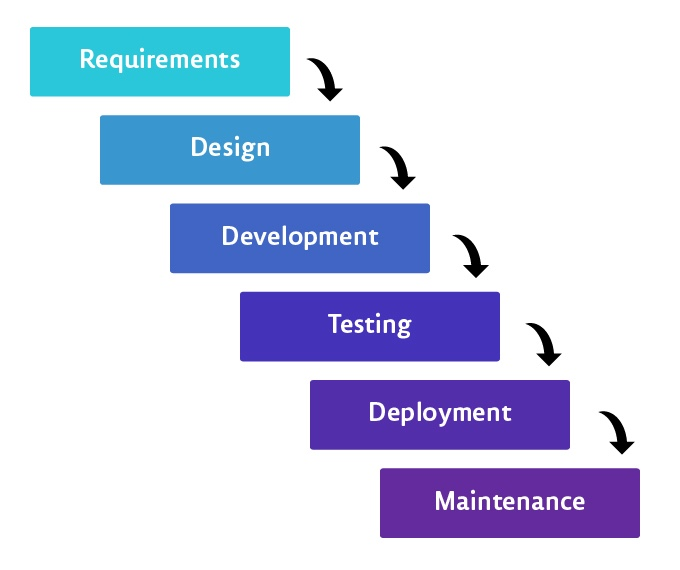
\includegraphics[width=0.5\textwidth]{../../img/chapter_2/sdlc-waterfall.jpg}
    \caption{Software Development Life Cycle - Waterfall Model}
    \label{fig:sdlc-waterfall}
\end{figure}

Today many SDLC models exist such as the Iterative Model, Spiral Model, V-Model, Big Bang Model, Agile Model, Software Prototype and Rapid Application Development Model. Each SDLC model comes with their own advantages and disadvantages, although this thesis will not be discussing those in depth. The objective of an SDLC model is to provide a structure for the different software development activities.  Albeit many models exist for the SDLC, it is generally divided in several phases including planning, defining requirements, design of software the architecture, development, and testing. A brief description of each phase is described below.

\paragraph{Planning}
Planning provides the foundation of every SDLC. The objective of the planning phase is to acquire the quality assurance, risk identification and feasibility report. 

\paragraph{Defining Requirements}
The next phase is centered on defining the details of the requirements gathered during the planning phase, document those and receive verification from the customer. The objective is the software development specification (SRS) document which comprises all the requirements of the product to be designed and developed.

\paragraph{Designing the Software Architecture}
Before actual development is started, the SRS is used as input to design several architectures of the software product. After reviewing the architectures the best design is selected. 

\paragraph{Development of the Product}
Based on the design of the previous phase, the actual development of the software product can begin.

\paragraph{Testing}
The final phase tests the developed software to assess whether it meets the user requirements defined in the SRS. If the tests are successful, the product can be deployed.

% \subsubsection{Agile Software Development}

% \subsection{Designing Secure Software}

% \subsubsection{Operation Security}\label{sec:opsec}
% Operation Security (OPSEC) is the analytical process as well a strategy utilized to identify information that potentially can be exploited by an attacker and used to collect vital information that could harm an organization's plans or reputation. Thus, OPSEC provides the means to design countermeasures to reduce or eliminate adversary exploitation.

% During the Vietnam War, a team dubbed Purple Dragon observed how their adversaries were able to anticipate their strategies and tactics despite North Vietnam and the Viet Cong's incapability to decrypt the United States communications. They concluded that the U.S. was unknowingly exposing information to the enemy that was being grouped together and exploited. The same theory has been brought over from the military to the information security professionals \cite{tunggal_what_2021}.

% \paragraph{The operation security process}
% The OPSEC process is a five-step risk assessment that assists in identifying what information needs to be protected, analyzing the threats and vulnerabilities that might impact, and develop mitigations for those threats and vulnerabilities as shown in Figure \ref{fig:opsec}.

% \begin{figure}[!h]
%     \centering
%     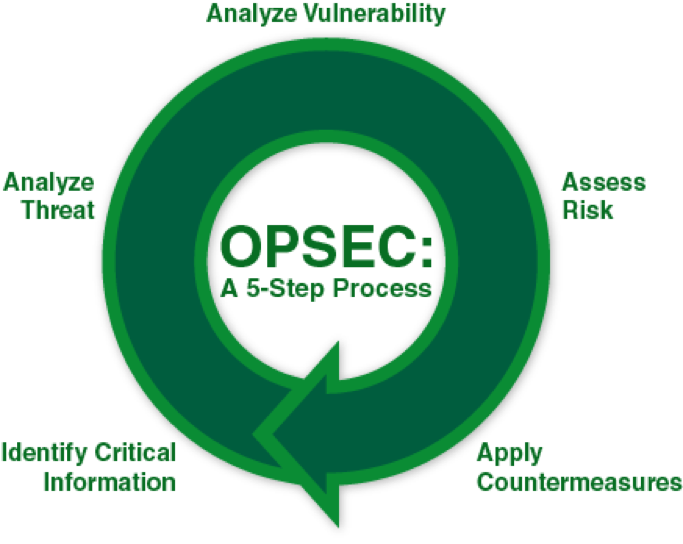
\includegraphics[width=.5\textwidth]{../../img/chapter_2/opsec-model.png}
%     \caption{OPSEC model}
%     \label{fig:opsec}
% \end{figure}

% \subparagraph{Identification of critical information}

% \subparagraph{Analysis of threats}

% \subparagraph{Analysis of vulnerabilities}

% \subparagraph{Assessment of risks}

